\newappendix\label{thirdappendix}
%\chapter{Appendix C: Benchmark Control Problems}
\section{Experiment 1: Automatic Cruise Control System for Cars\cite{Murray2009}}
\subsection{Aim}
To design and develop a cruise control system of a car.
\subsection{System Modeling}
Consider a vehicle of mass \textit{m} moving at a velocity \textit{v}. A force \textit{F} is generated from the engine while a disturbance force $ F_d $ is resisting motion of the vehicle \cite{Murray2009,koruba2012classical}. Therefore, the equation of motion of the vehicle is given by
\begin{equation} \label{eq:force}
m\frac{{dv}}{{dt}} = F - {F_D}
\end{equation}
The vehicle engine generates force \textit{F} which is proportional to the rate of injected fuel in the engine. This phenomenon in turn controls the throttle of the vehicle. Torque produced $ T $ at engine speed $ \omega $ can be mathematically represented as
\begin{equation}
T\left( \omega  \right) = {T_m}\left( {1 - \beta {{\left( {\frac{\omega }{{{\omega _m}}} - 1} \right)}^2}} \right)
\end{equation} 
where $ T_m $ is maximum torque generated by the engine at full throttle to attain $ \omega _m $, the maximum engine speed with torque coefficient $ \beta $. For a gear ratio \textit{n} and wheel radius \textit{r}, current velocity can be related to the engine speed by \eqref{eq:1}
\begin{equation} \label{eq:xx1}
\omega  = \frac{n}{r}v = {\alpha _n}v
\end{equation}
Therefore the driving force can be computed as
\begin{equation} \label{eq:F}
F = \frac{{nu}}{r}T\left( \omega  \right) = {\alpha _n}uT\left( {{\alpha _n}v} \right)
\end{equation}
Basically there are three major disturbance forces working on the vehicle namely, gravitational force ($ F_G $), rolling friction of the road and vehicle tires ($ F_R $), and aerodynamic drag due to the body of the vehicle ($ F_A $).
\begin{equation} \label{eq:2}
{F_D} = {F_G} + {F_R} + {F_A}
\end{equation}
The gravitational force acting on the vehicle can be modeled based on the slope of the roads.
\begin{align} \label{eq:3}
{F_G} &= mg\sin \theta \\
{F_R} &= mgC_r sgn\left(v\right) \\
{F_A} &= \frac{1}{2}\rho {C_d}A{v^2}
\end{align}
Combining \eqref{eq:2} and \eqref{eq:3}, \eqref{eq:force} becomes
\begin{align} \label{eq:Tforce}
m\frac{{dv}}{{dt}} &= {\alpha _n}uT\left( {{\alpha _n}v} \right) -  mg\sin \theta - \\
& mg{C_r}{\mathop{\rm sgn}} ( v ) - \frac{1}{2}\rho {C_d}A{v^2} \nonumber 
\end{align}

\subsection{Controller Design and Tuning}
A PI controller was used to benchmark the performance of this control problem. The designed PI controller was tuned using Ziegler-Nichols method with help of Matlab Control System Toolbox. The controller gains are specified in Table \ref{tab:Gain_ACC}.

\begin{table}[h]
	\centering
	\caption{Proportional and Integral Gains in ACC System}
	\label{tab:Gain_ACC}
	\begin{tabular}{ll} 
		\hline
		Gain & Value \\ \hline
		$ K_P $ & 0.1   \\
		$ K_I $ & 0.5  \\ \hline
	\end{tabular}
\end{table}

\section{Experiment 2: Two Tank Water Level Control \cite{Laubwald2006}}
\subsection{Aim}
To control water level in a coupled tank.
\subsection{System Modeling}
Consider the coupled tank system in Figure \ref{fig:CoupledTank}. The system comes from two flow balances and the non-linear equations for flow appear through the valves. When the valves are assumed to have ideal orifice, the system nonlinearity is described by square root law. The flow balance equations are,
\[\begin{array}{l}
{Q_i} - {C_{db}}{a_b}\sqrt {2g({H_1} - {H_2})}  = A\frac{{d{H_1}}}{{dt}}\\
{C_{db}}{a_b}\sqrt {2g({H_1} - {H_2})}  - {C_{db}}{a_b}\sqrt {2g{H_2}}  = A\frac{{d{H_2}}}{{dt}}
\end{array}\]

\begin{figure}
\centering
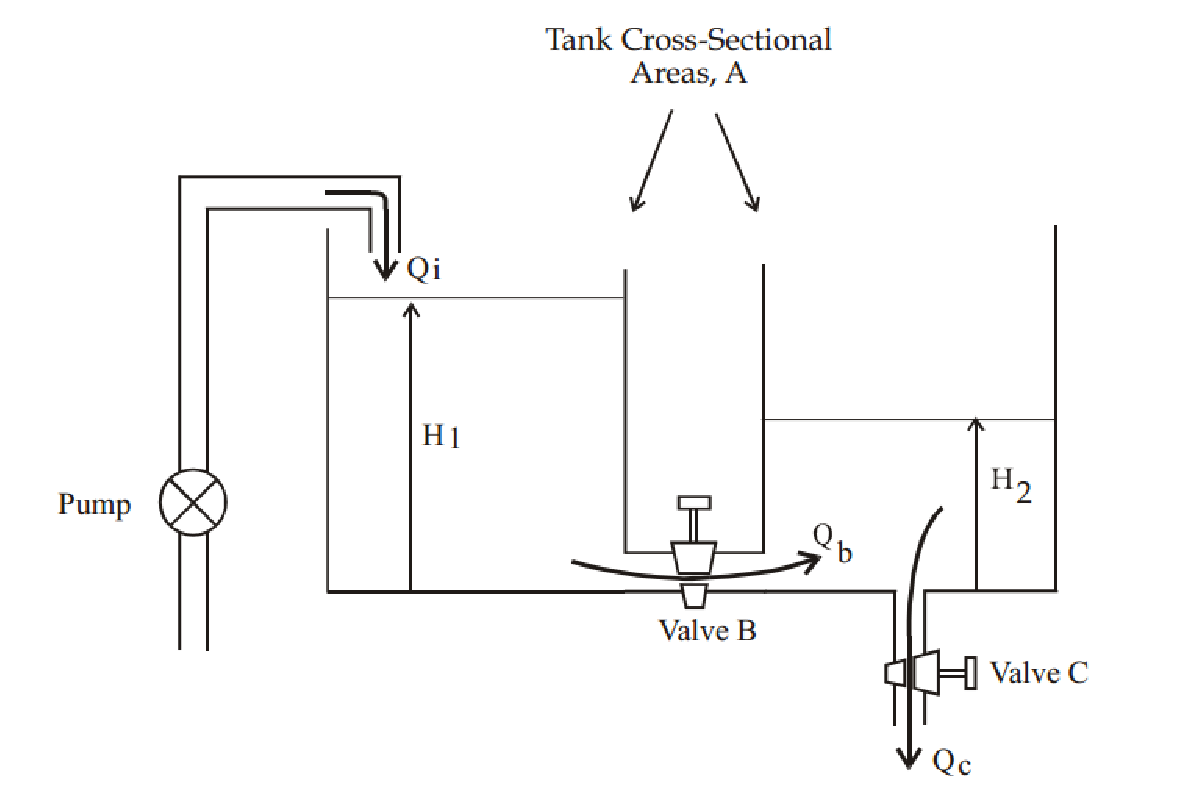
\includegraphics[width=0.7\linewidth]{Appendix3/CoupledTank}
\caption{Coupled Tanks System \cite{Laubwald2006}}
\label{fig:CoupledTank}
\end{figure}


\subsection{Controller Design and Tuning}
For the controller design, the above equations are linearized. This is done assuming small variations in $q_i$ in $Q_i$, $h_1$ in $H_1$, $h_2$ in $H_2$. After linearizing of the above equations can be presented as,
\[\begin{array}{l}
\left[ {\begin{array}{*{20}{c}}
	{{{\dot x}_1}}\\
	{{{\dot x}_2}}
	\end{array}} \right] = \left[ {\begin{array}{*{20}{c}}
	{{k_{11}}}&{{k_{12}}}\\
	{{k_{21}}}&{{k_{22}}}
	\end{array}} \right]\left[ {\begin{array}{*{20}{c}}
	{{x_1}}\\
	{{x_2}}
	\end{array}} \right] + \left[ {\begin{array}{*{20}{c}}
	{{A^{ - 1}}}\\
	0
	\end{array}} \right]{q_i}\\
\left[ {\begin{array}{*{20}{c}}
	{{h_1}}\\
	{{h_2}}
	\end{array}} \right] = \left[ {\begin{array}{*{20}{c}}
	1&0\\
	0&1
	\end{array}} \right]\left[ {\begin{array}{*{20}{c}}
	{{x_1}}\\
	{{x_2}}
	\end{array}} \right]
\end{array}\]

The transfer function model is as follows
\[\frac{{{h_2}(s)}}{{{q_i}(s)}} = \frac{G}{{\left( {{T_1}s + 1} \right)\left( {{T_2}s + 1} \right)}}\]

Implementing a PI controller,
\[y(s) = \frac{{g({k_i} + {k_p}s)r(s)}}{{T{s^2} + s(1 + g{k_p}) + g{k_i}}} + \frac{{(gs)d(s)}}{{T{s^2} + s(1 + g{k_p}) + g{k_i}}}\]

With natural frequency of 0.01 Hz and a damping factor of 1, the control system parameters were set up to be $ {k_i}=0.1 $ and $ {k_p}=2.7 $


\section{Experiment 3: Armature Controlled DC Motor\cite{malla2012}}
\subsection{Aim}
To control speed of a DC motor.
\subsection{System Modeling}
Consider the Figure \ref{fig:ACDC_motor_01}, which shows the operation of an Armature controlled DC motor \cite{malla2012,MathworksInc.2014}.
\begin{figure}
\centering
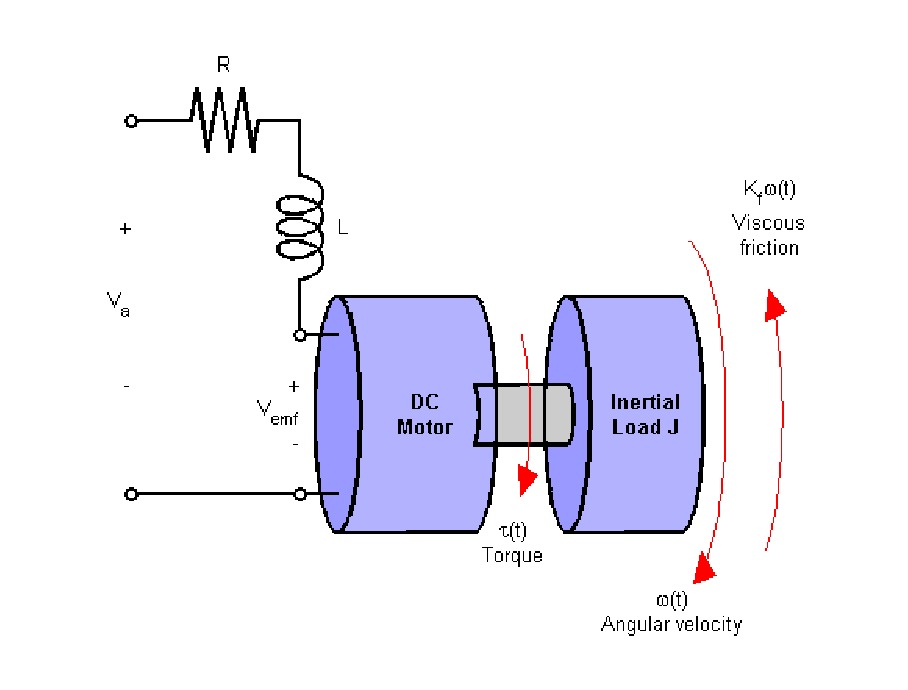
\includegraphics[width=0.7\linewidth]{Appendix3/ACDC_motor_01}
\caption{Armature Controlled DC Motor}
\label{fig:ACDC_motor_01}
\end{figure}

The physical constants of the control problem are 
Armature Resistance $ (R_A) $ = 1 $\Omega $, 
Armature Inductance $ (L_A) $ = 0.5, 
Inertia $ (J_M) $ = 0.01, 
Damping $ (B_M) $ = 0.1, 
Torque Constant $ (K_{\tau}) $  0.01 Nm/A and 
Back EMF Constant $ (K_B) $ = 0.01 Vs/rad. 

Transfer function of the plant model is stated as,
\begin{align} 
\frac{\theta {\rm (}s{\rm )}}{V_A{\rm (}s{\rm )}}{\rm =\ } \frac{K_{\tau }}{L_AJ_Ms^{{\rm 3}}{\rm +}\left(R_AJ_M{\rm +}L_AB_M\right)s^{{\rm 2}}} \nonumber\\
{\rm x\ } \frac{1}{\left(K_{\tau }K_B{\rm +}R_AB_M\right)s}
\end{align}


\subsection{Controller Design and Tuning}

The above model is loaded with Torque $T_D$. A PID controller is employed to obtain a smooth control of the Armature Controlled DC motor. The controller is tuned using Mathworks Systune PID Tuner. The controller gains are tabulated in Table \ref{tab:ACDC_gain}.

\begin{table}[]
	\centering
	\caption{Controller Gains in Speed Control of Armature Controlled DC Motor}
	\label{tab:ACDC_gain}
	\begin{tabular}{ll}\\
		\hline
		Gain & Value \\ \hline
		$ K_P $ & 17.94 \\
		$ K_I $ & 43.45 \\
		$ K_D $ & -0.78 \\ \hline
	\end{tabular}
\end{table}


